\documentclass{csse4400}

% \teachermodetrue

\usepackage{languages}
\usepackage{float}

\title{Deploying with Terraform}
\author{Brae Webb}

\date{\week{3}}
\begin{document}

\maketitle

\section{Before Class}
Ensure you've had practice using the AWS Academy learner lab.
It's preferable if you already have \link{terraform installed}{https://learn.hashicorp.com/tutorials/terraform/install-cli}.
Please also have one of IntelliJ IDEA, PyCharm, or VSCode with the terraform plugin installed.

\noindent It is also helpful to have read the Infrastructure as Code lecture notes to understand the motivation for using a tool like Terraform.

\section{This Week}
This week we are going to put our Terraform and AWS knowledge together to deploy our Todo Application.
Specifically, this week you need to:
\begin{itemize}
    \item Authenticate Terraform to use the AWS learner lab.
    \item Configure an RDS database and use it in the Todo Application.
    \item Configure a single server website in Terraform and deploy the Todo Application to it.
\end{itemize}

\section{Using Terraform in AWS Learner Labs}
Following the steps from the week four practical, start a learner lab in AWS Academy.
For this practical, you do not need to create any resources in the AWS Console.
The console can be used to verify that Terraform has correctly provisioned resources.

\begin{enumerate}
\item Once the learner lab has started, click on `AWS Details' to display information about the lab.

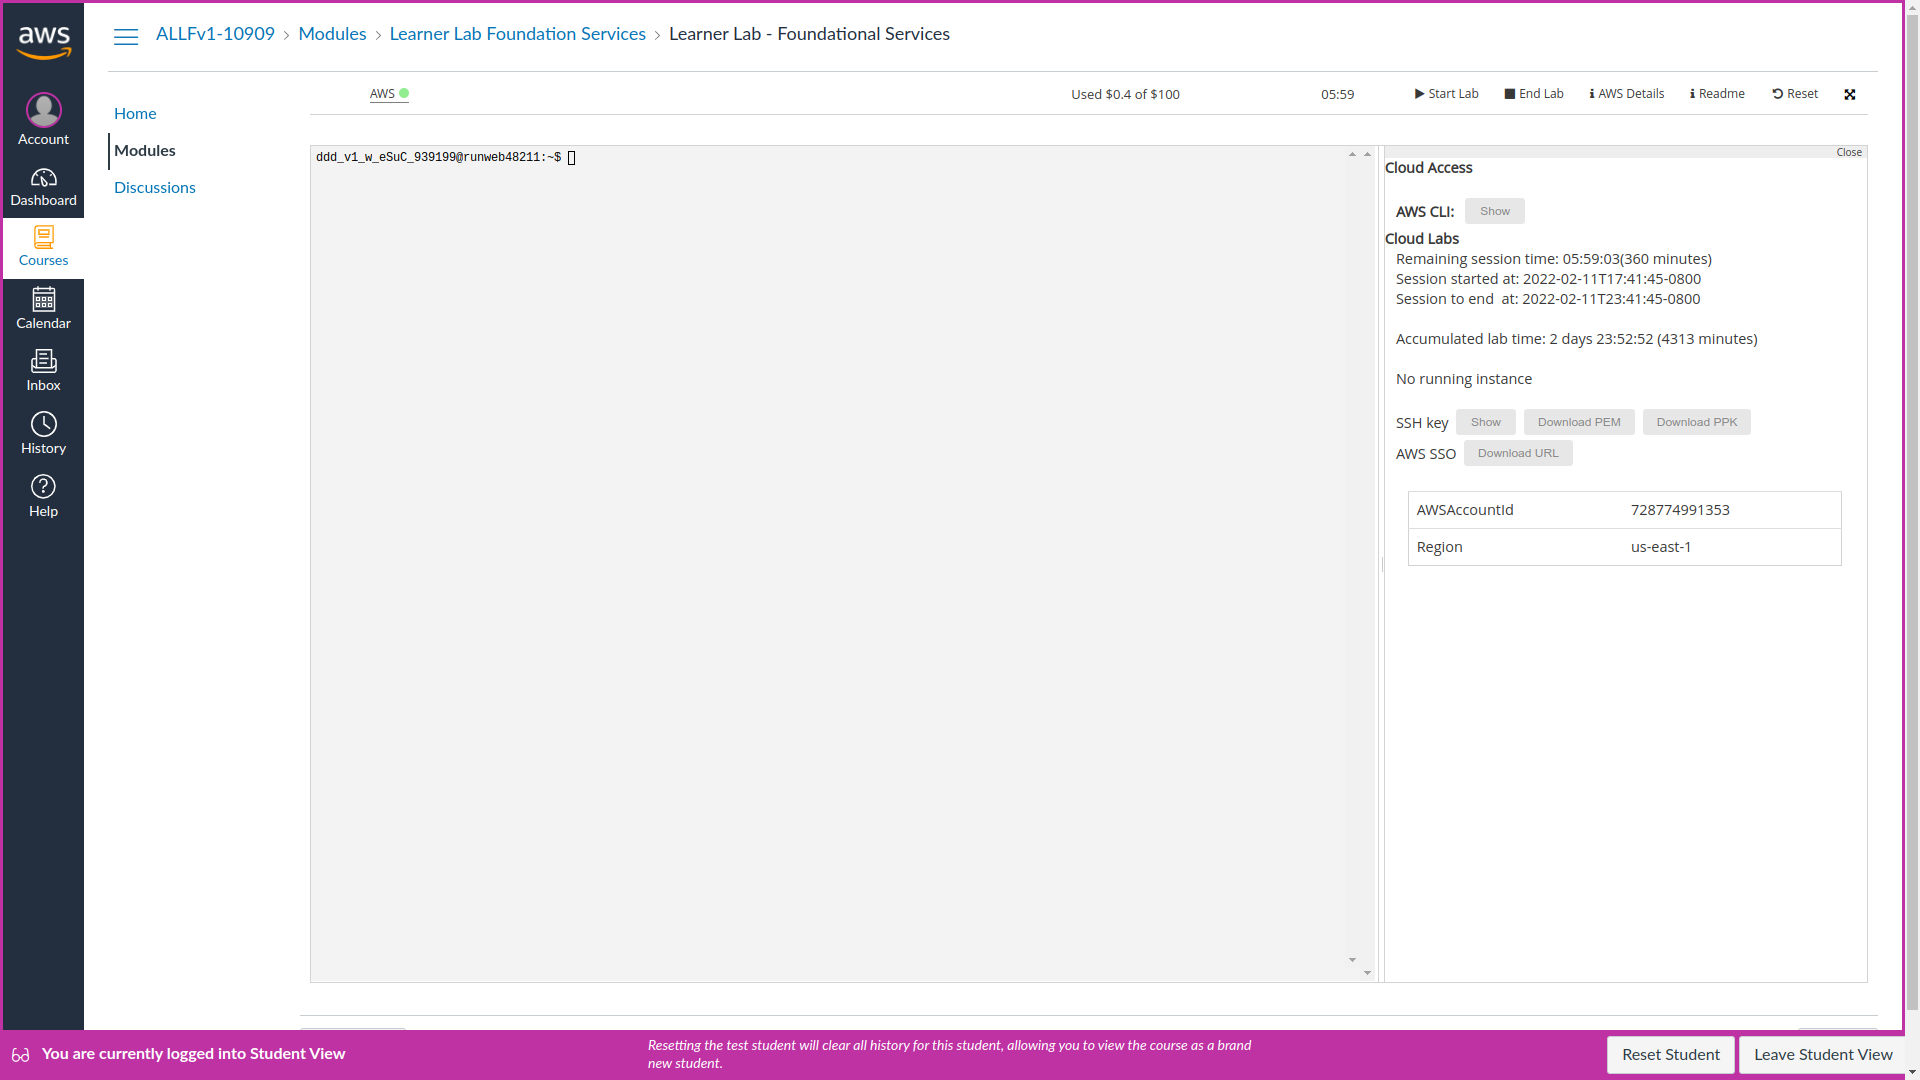
\includegraphics[width=0.7\textwidth]{images/aws-details}

\item Click on the first `Show' button next to `AWS CLI' which will display a text block starting with \texttt{[default]}.
\item Create a directory for this week's practical.
\item Within that directory create a \texttt{credentials} file and copy the contents of the text block into the file.
\textbf{Do not share this file contents --- do not commit it}.
\item Create a \texttt{main.tf} file in the same directory with the following contents:
\begin{code}[language=terraform]{main.tf}
terraform {
    required_providers {
        aws = {
            source  = "hashicorp/aws"
            version = "~> 3.0"
        }
    }
}

provider "aws" {
    region = "us-east-1"
    shared_credentials_file = "./credentials"
}
\end{code}

The \texttt{terraform} block specifies the required external dependencies, here we need to use the AWS provider.
The \texttt{provider} block configures the AWS provider, instructing it which region to use and how to authenticate (using the credentials file we created).

\item We need to initialise terraform which will fetch the required dependencies. This is done with the \texttt{terraform init} command.
\bash{terraform init}

This command will create a \texttt{.terraform} directory which stores providers and a provider lock file, \texttt{.terraform.lock.hcl}.

\item To verify that we have setup Terraform correctly, use \texttt{terraform plan}.
\bash{terraform plan}

As we currently have no resources configured, it should find that no changes are required.
Note that this does not ensure our credentials are correctly configured as Terraform has no reason to try authenticating yet.

\end{enumerate}

\section{Deploying a Database in AWS}

\info{
  This section manually deploys a Postgresql RDS instance, which is not the courses end goals but is a good way to get started with AWS. Latter this practical we will use terraform to create the database, so this section is optional and is better to be observed rather than actioned.
}

\teacher{
  Instruct the class to observe you making the database and not to follow along.
}

\begin{figure}[ht]
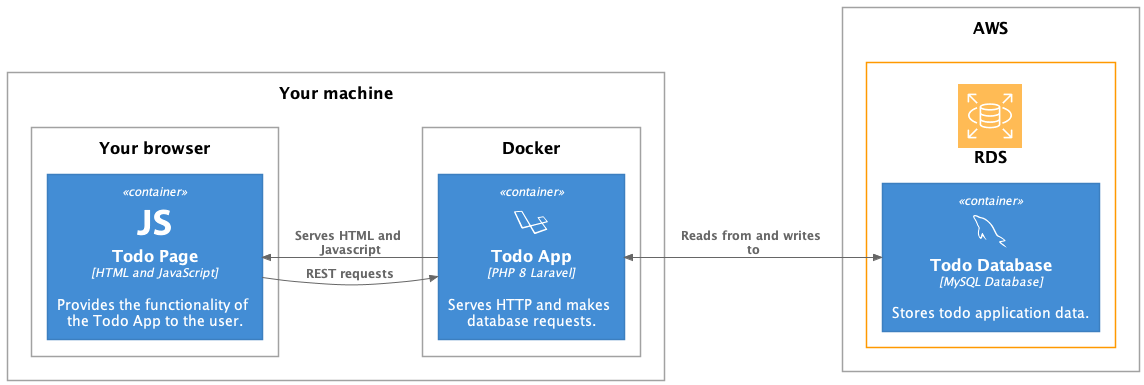
\includegraphics[width=\textwidth]{diagrams/remotedb}
\caption{Remote database deployment diagram}
\end{figure}

Now we have a locally running Todo App let's move to AWS, start up your Learner Lab environment now.

This is the last time we will heavily use the AWS user interface in the practicals. If you already feel confident in the AWS environment skip to Section \ref{sect:terraform} for the terraform setup.

\teacher{
  Give students time to start the labs, could take up to 10 minutes.
}

To get started let's jump into the lab environment and have a look at AWS RDS which is an AWS managed database service. To get to the RDS service either search it or browse Services -> Database -> RDS as shown below.

\begin{figure}[H]
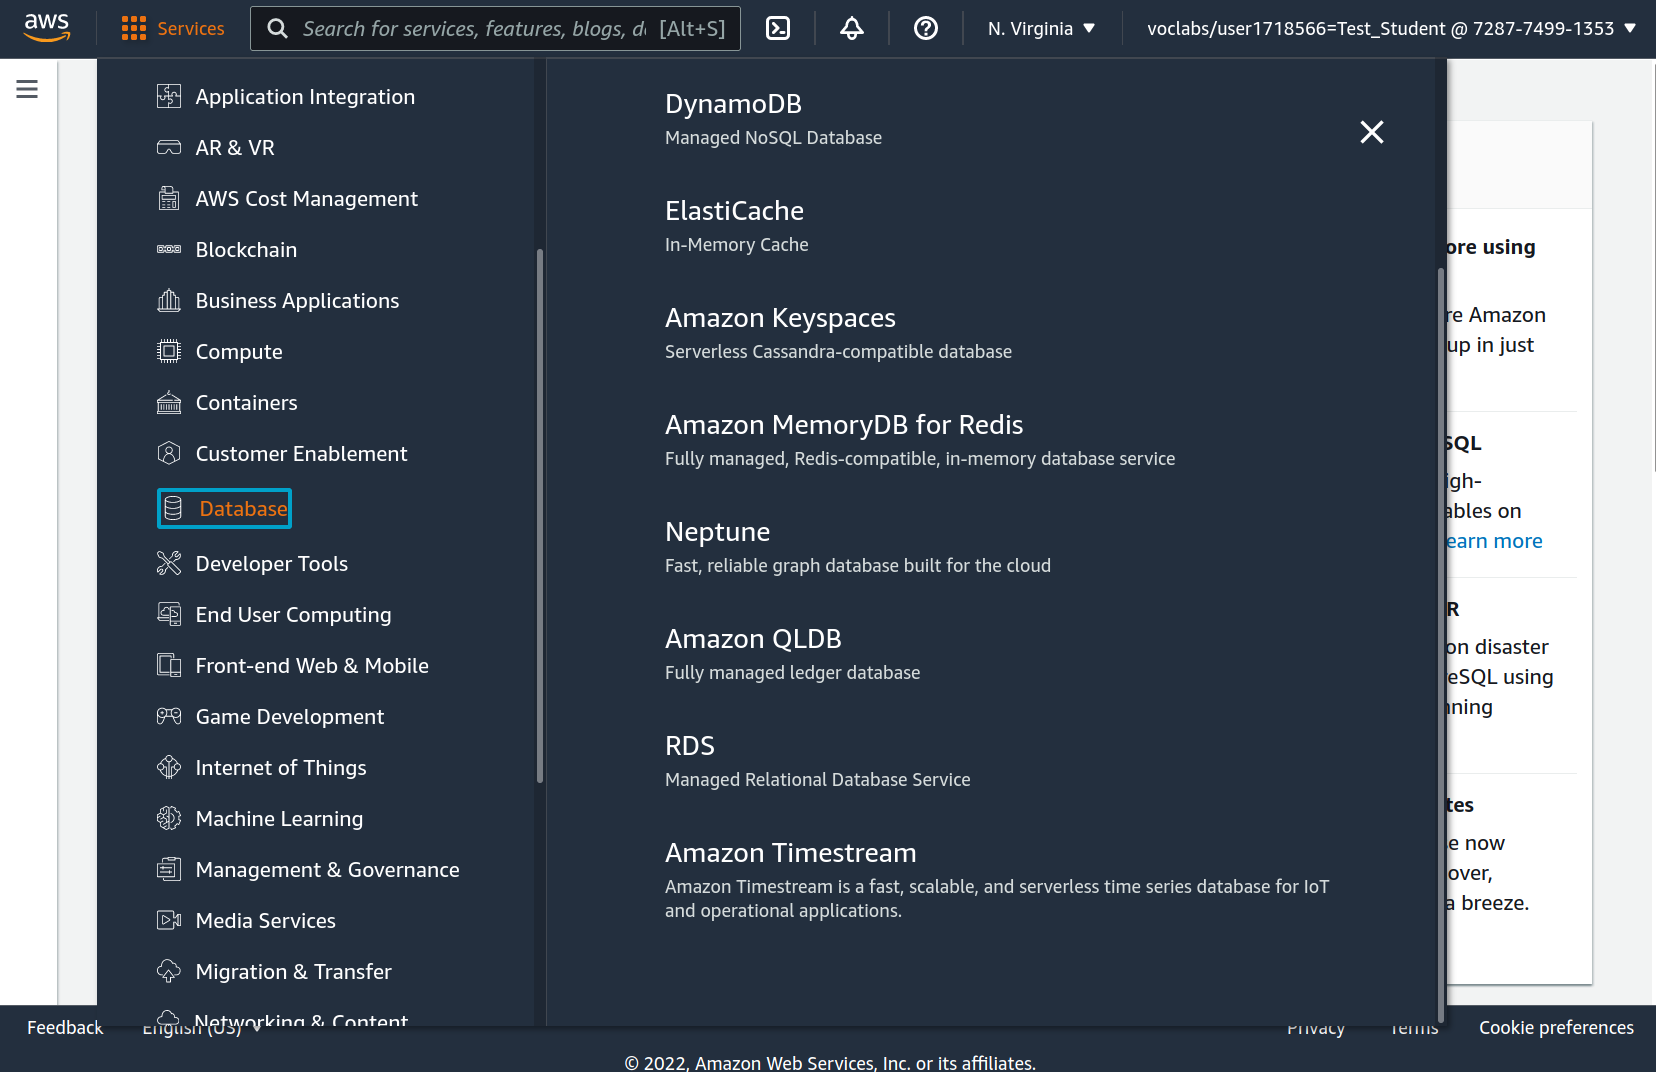
\includegraphics[width=\textwidth]{images/aws_1}
\end{figure}

Now we are in the management page for all our database instances,
for today we just want to get a small instance running to explore the service.
Head to ``DB Instances (0/40)''.

\begin{figure}[H]
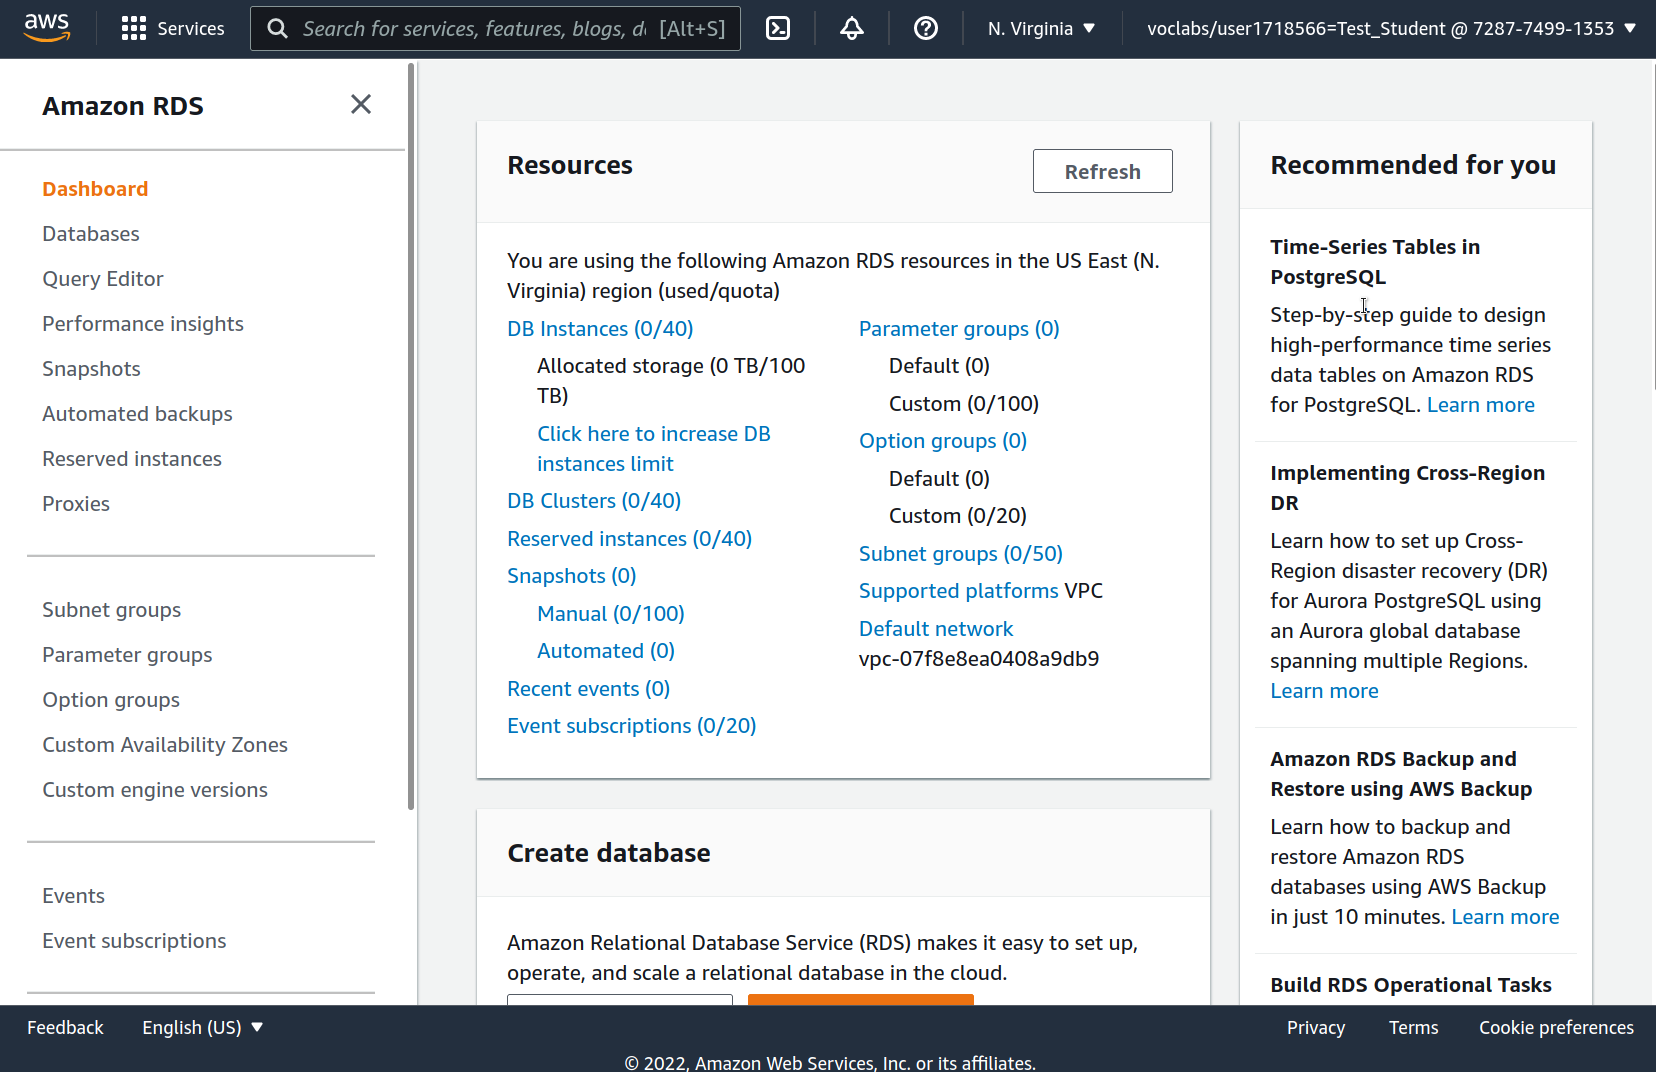
\includegraphics[width=\textwidth]{images/aws_2}
\end{figure}

This page should appear familar as it's very similar to the AWS EC2 instance page.
Let us create a new database by hitting the ``Create Database'' button.

\begin{figure}[H]
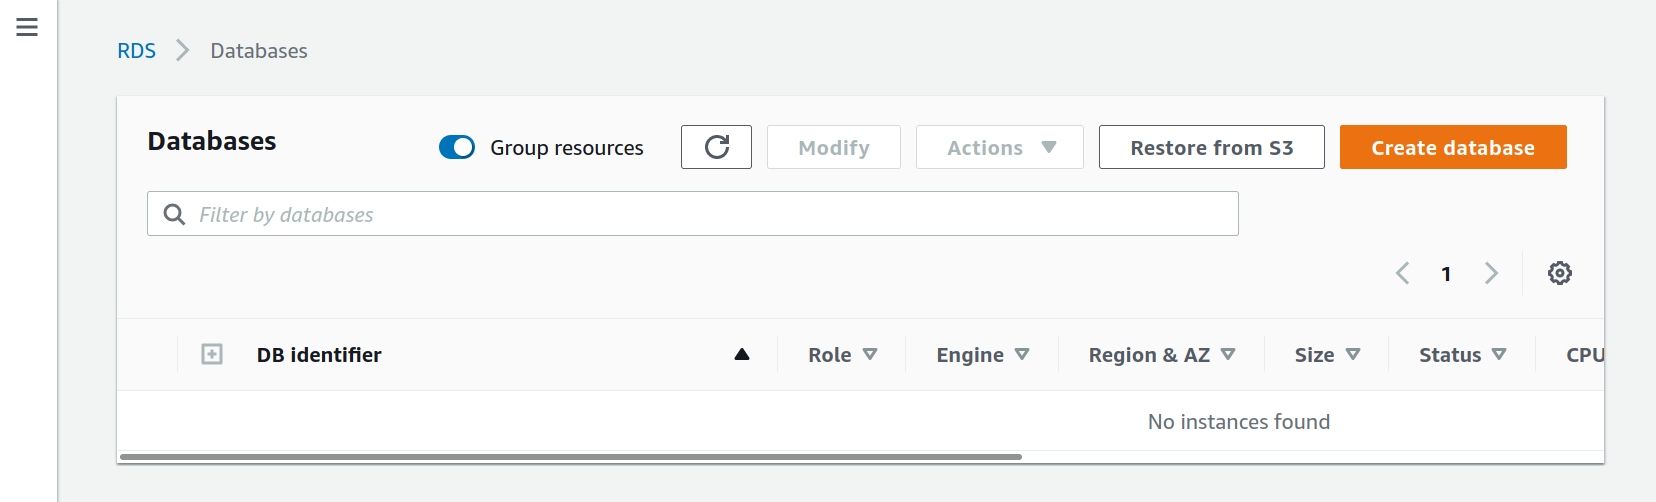
\includegraphics[width=\textwidth]{images/aws_3}
\end{figure}

\warning{
  In the next section we cannot use the Easy Create method as it tries to create a IAM account which is not allowed in the labs.
  Going forward we would typically do this using Terraform so we can easily avoid these restrictions.
}

\teacher{
  Feel free to talk about the other offerings here, but make sure to flame Oracle and Microsoft SQL Server.
  A good thing to point out is the Amazon Aurora which is the serverless version of RDS.
}

We will be creating a standard database so select standard and MySQL.
We will use version 8 to match the local version.

\begin{figure}[H]
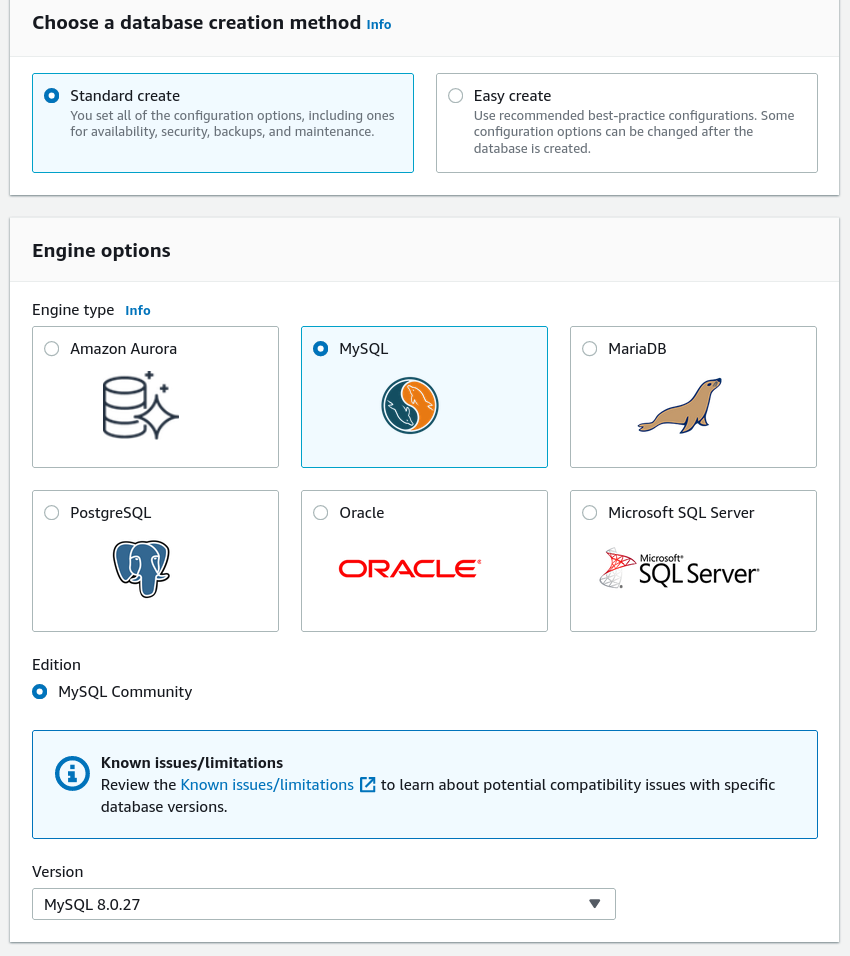
\includegraphics[width=\textwidth]{images/db1}
\end{figure}

For today we are going to use ``Free Tier'' but in the future,
you may wish to explore the different deployment options.
Please peruse the available different options.

\teacher{
  Walk through what Multi-AZ means aka Multiple Availability Zones.
}

\begin{figure}[H]
  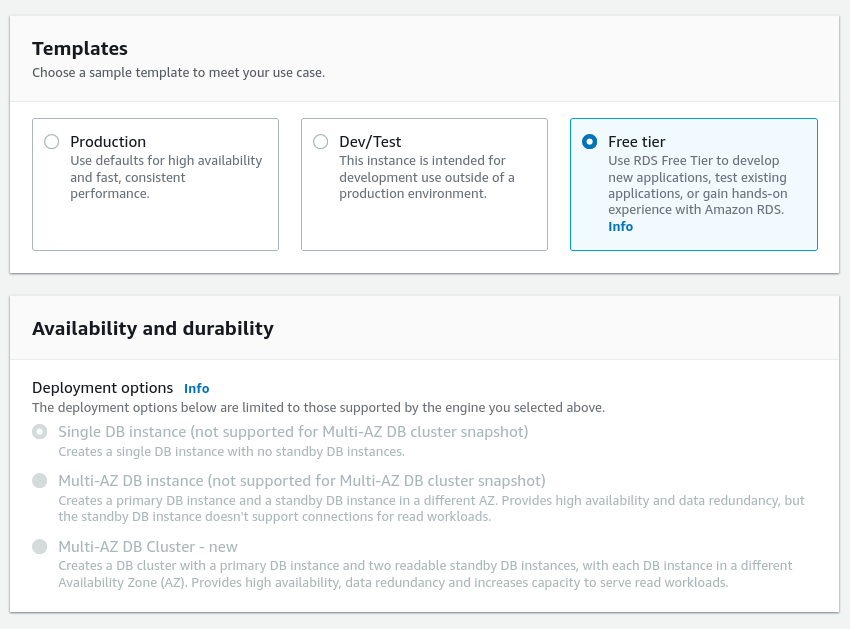
\includegraphics[width=\textwidth]{images/db2}
\end{figure}

Now we need to name our database and create credentials to connect via.
Please enter a reasonable password and keep this aside for later.
We will need it for our local docker-compose file.

\begin{figure}[H]
  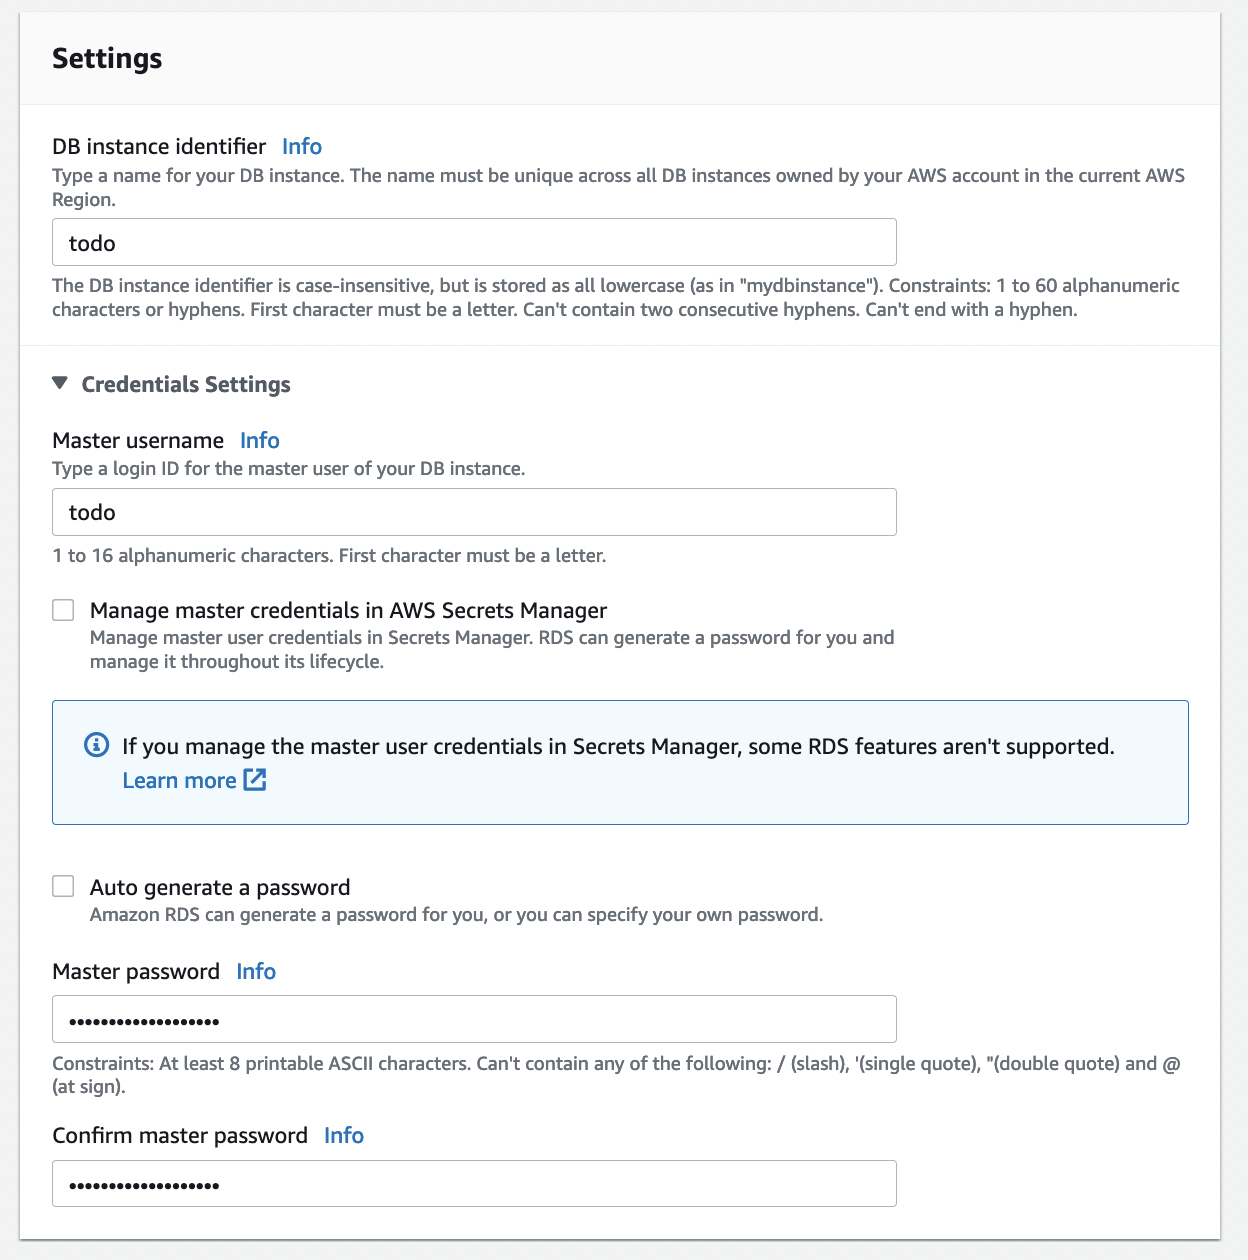
\includegraphics[width=\textwidth]{images/db3}
\end{figure}

We will use the default class type, t2.micro, which should be sufficient for this practical.

\teacher{
  May want to mention that burstable is not recommended for consistantly used databases.
  Usually DBs are memory focused and thus the standard or memory optimised are used.
}

\begin{figure}[H]
  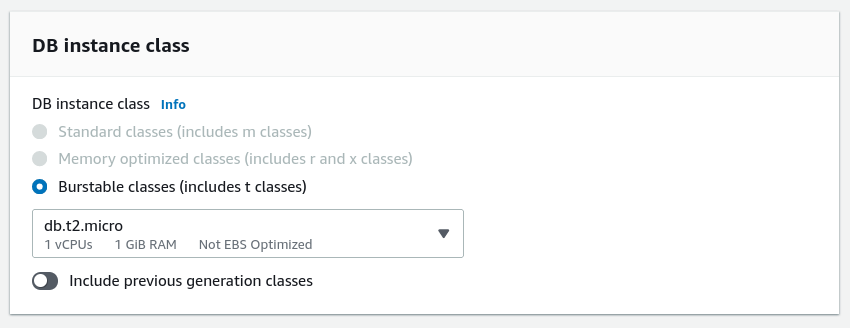
\includegraphics[width=\textwidth]{images/db4}
\end{figure}

For storage we will leave all the default options.

\begin{figure}[H]
  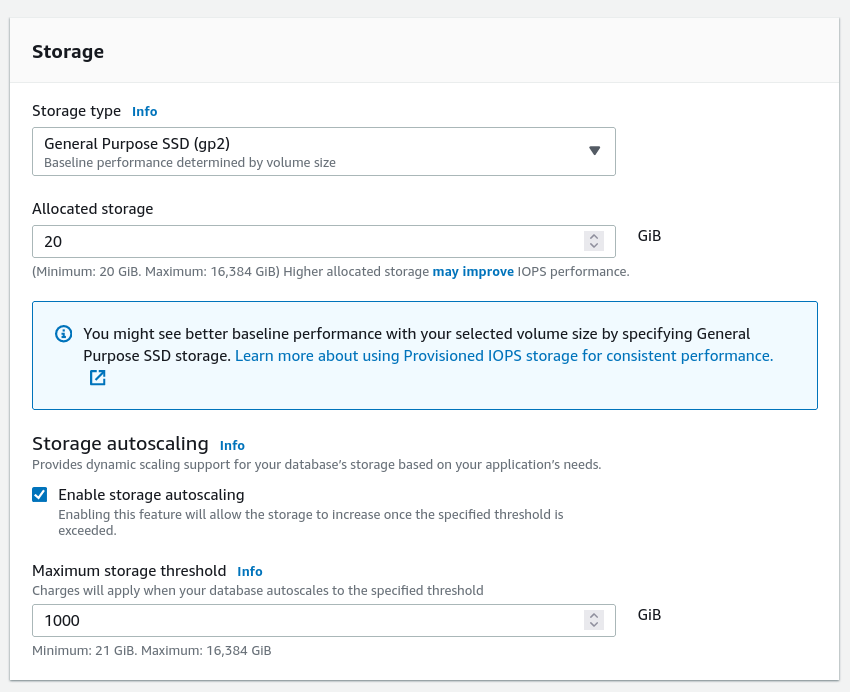
\includegraphics[width=\textwidth]{images/db5}
\end{figure}

In connectivity we need to make sure our instance is publicly available.
Usually you don't want to expose your databases publicly and, would instead, have a web server sitting in-front.
But for today we will be running that web server locally so for convenience we need public access.

When selecting public access as yes we have to create a new Security Group,
give this Security Group a sensible name.

\begin{figure}[H]
  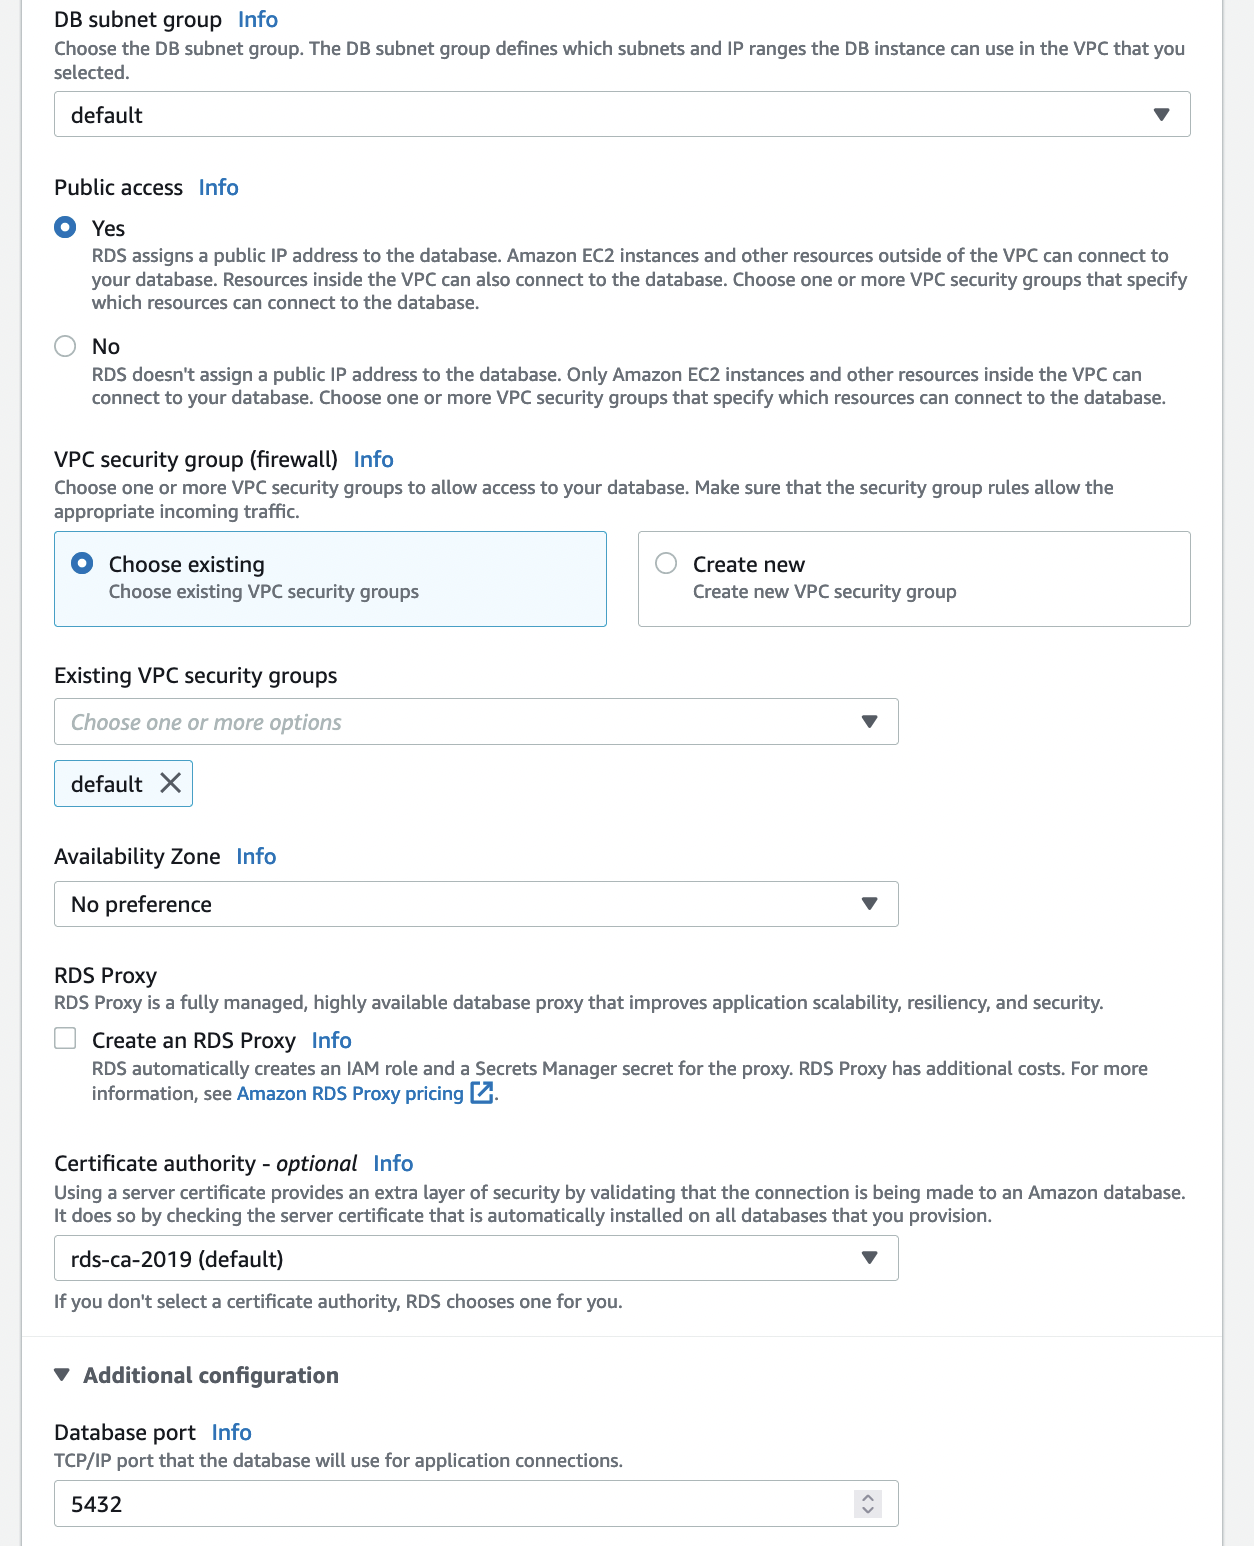
\includegraphics[width=\textwidth]{images/db6}
\end{figure}

We will leave the authentication as password based but we need to expand the ``Additional configuration''.
Fill in the ``Initial Database Name'' section to be ``todoapp'',
this is similar to what we had in the Docker Compose.

\teacher{
The other options here are to do with the parameters used to start the database,
it is uncommon to have to change these but this is where any settings you would pass in via cli to the db would be set.
}

\begin{figure}[H]
  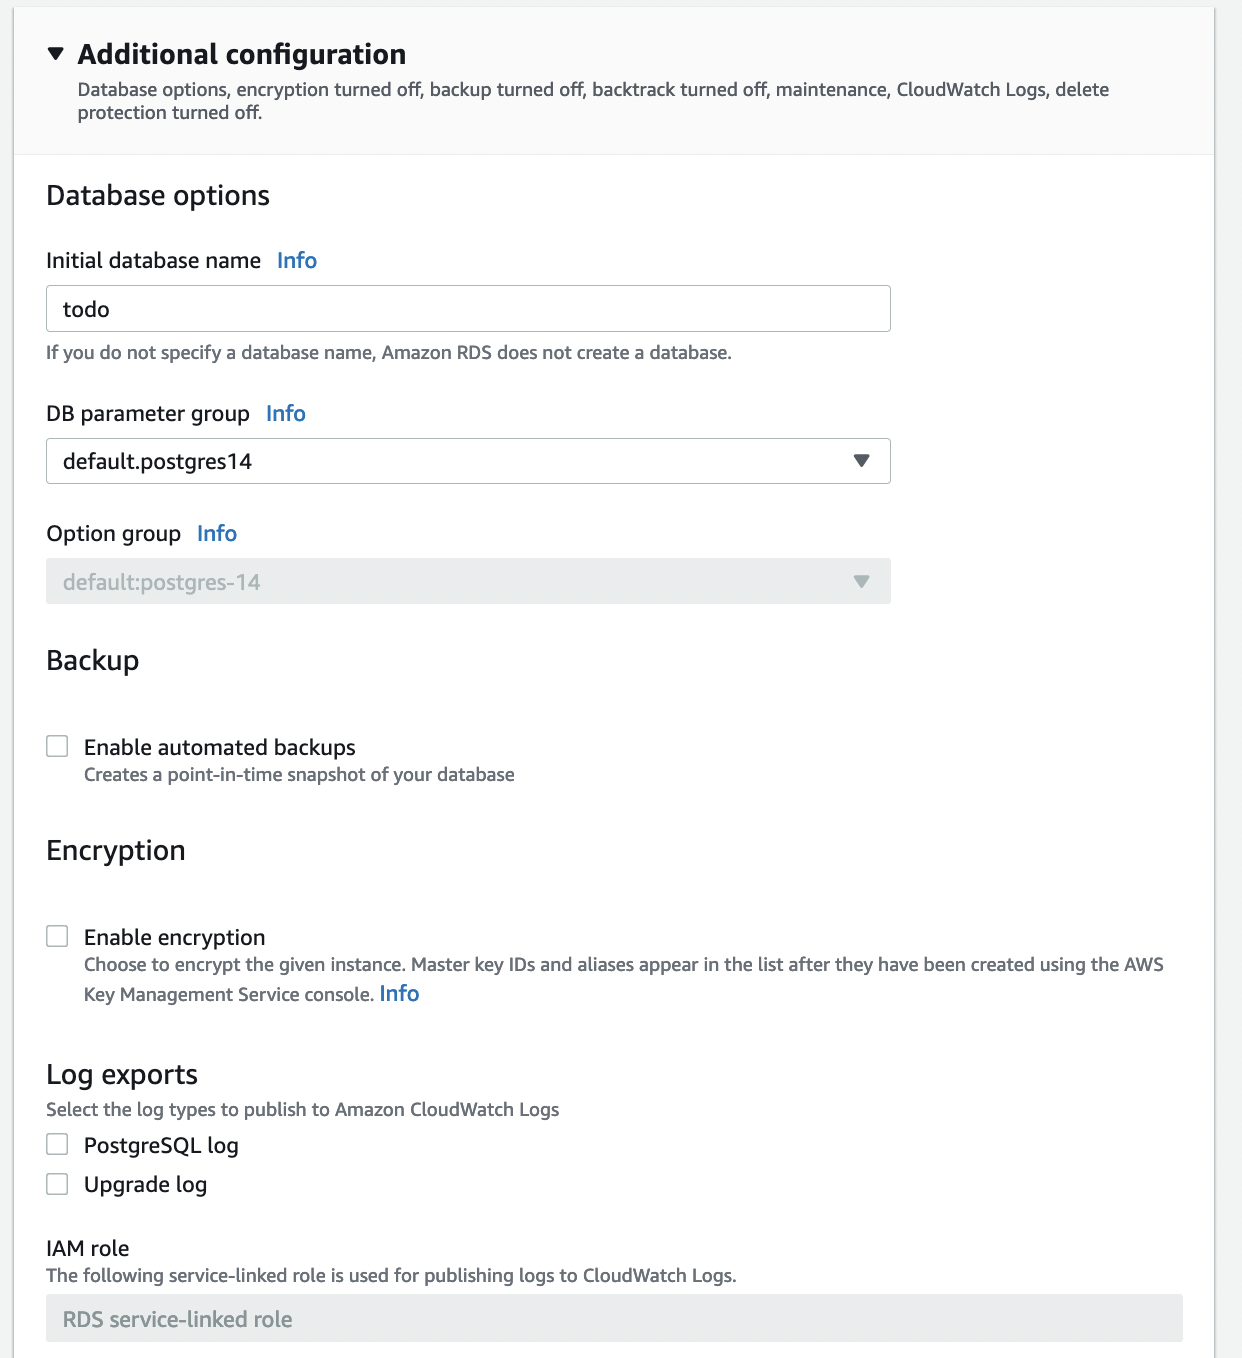
\includegraphics[width=\textwidth]{images/db7}
\end{figure}

Now we can click create which will take some time.

\begin{figure}[H]
  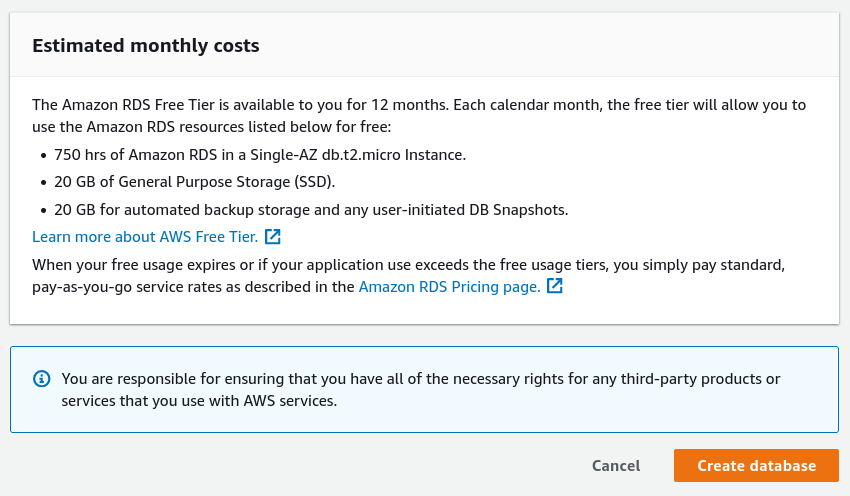
\includegraphics[width=\textwidth]{images/db8}
\end{figure}

Depending on your database it may take 10 to 30minutes to create,
the larger and more complicated the setup the longer it usually takes.
The database will also do a initial backup when its created.

\begin{figure}[H]
  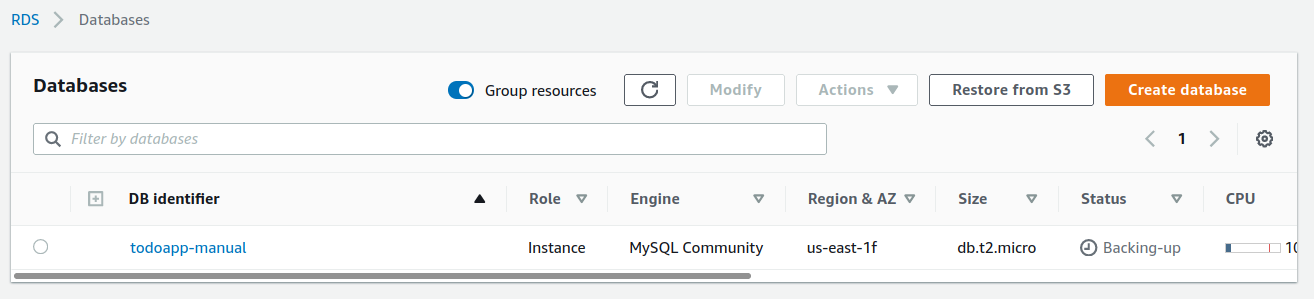
\includegraphics[width=\textwidth]{images/aws_4}
\end{figure}

When the database has finished being created you can select it to view the configuration and details.
In this menu we also see the endpoint address which we will need to copy into our docker compose file.

\begin{figure}[H]
  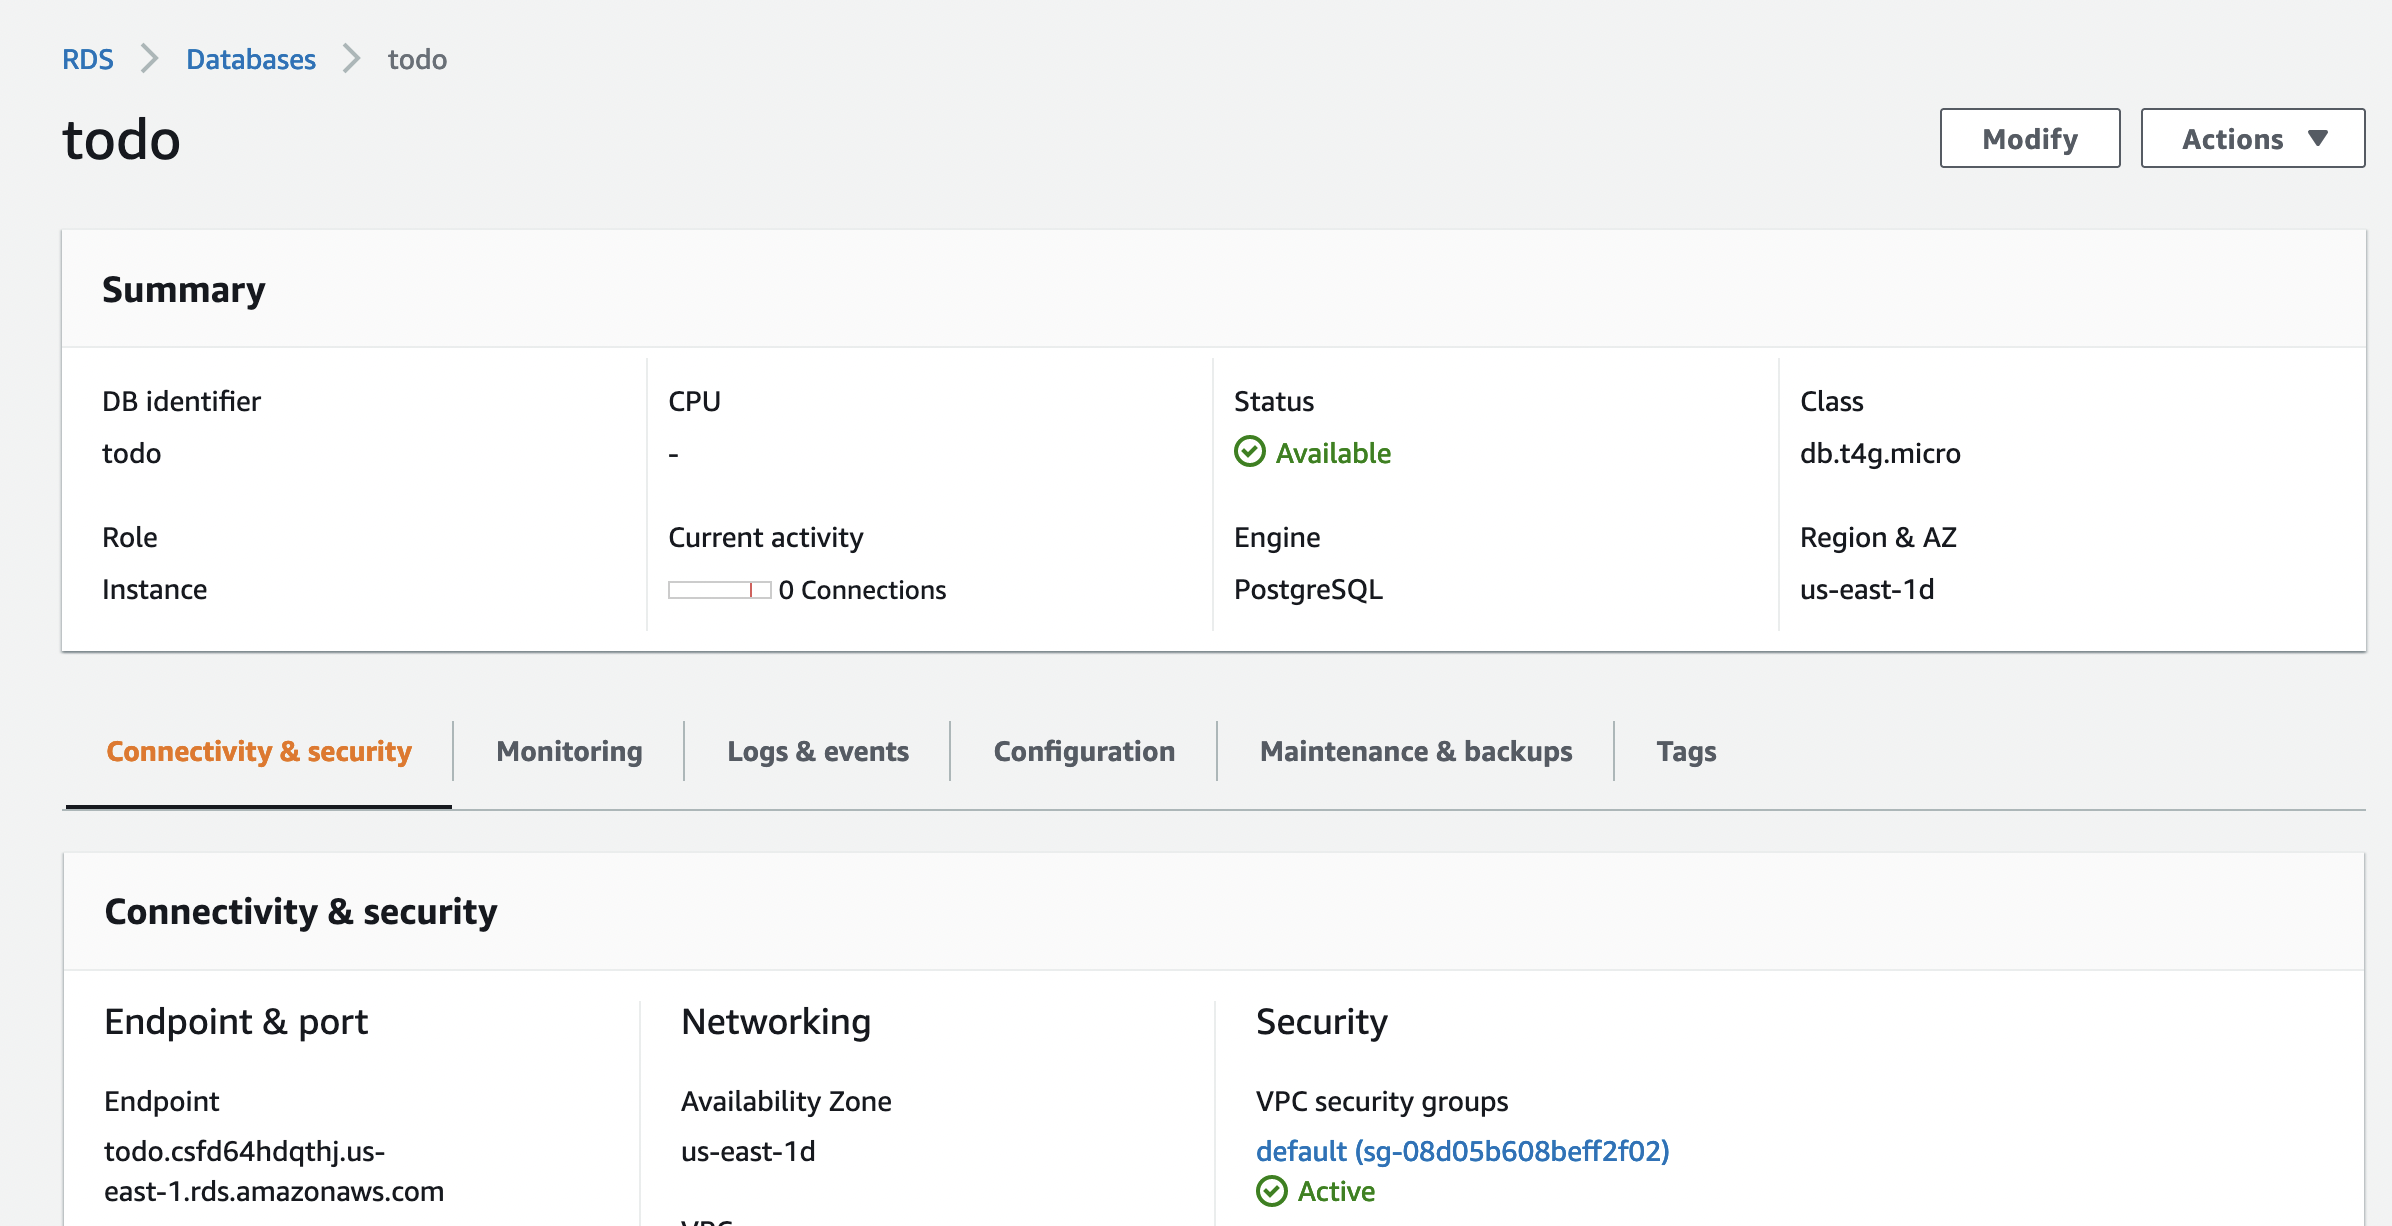
\includegraphics[width=\textwidth]{images/aws_5}
\end{figure}

\section{RDS Database with Terraform}

Now would be a good time to browse the documentation for the RDS database in Terraform:
\url{https://registry.terraform.io/providers/hashicorp/aws/latest/docs/resources/db_instance}.
Using our manual configuration,
we can come up with a resource with the appropriate parameters as below:

\begin{code}[language=terraform]{main.tf}
locals {
  password = "foobarbaz" # this is bad
}

resource "aws_db_instance" "todoapp-database" {
  allocated_storage      = 20
  max_allocated_storage  = 1000
  engine                 = "mysql"
  engine_version         = "8.0.27"
  instance_class         = "db.t2.micro"
  name                   = "todoapp"
  username               = "todoapp"
  password               = local.password
  parameter_group_name   = "default.mysql8.0"
  skip_final_snapshot    = true
  vpc_security_group_ids = [aws_security_group.todoapp-database.id]
  publicly_accessible    = true

  tags = {
    Name = "todoapp-database"
  }
}
\end{code}

\noindent Remember to create an appropriate security group as we did through the user interface.

\begin{code}[language=terraform]{main.tf}
resource "aws_security_group" "todoapp-database" {
  name        = "todoapp-database"
  description = "Allow inbound MySQL traffic"

  ingress {
    from_port        = 3306
    to_port          = 3306
    protocol         = "tcp"
    cidr_blocks      = ["0.0.0.0/0"]
  }

  egress {
    from_port        = 0
    to_port          = 0
    protocol         = "-1"
    cidr_blocks      = ["0.0.0.0/0"]
    ipv6_cidr_blocks = ["::/0"]
  }

  tags = {
    Name = "todoapp-database"
  }
}
\end{code}

\todo{Add a section where we connect to the database using our locally running todo app.}

\section{Container on AWS}

As we mentioned in the Infrastructure as Code notes \cite{iac-notes},
in this course we will use Docker to configure machines and Terraform to configure infrastructure.
AWS has the ability to deploy Docker containers using a service known as Elastic Container Service (ECS).
Unfortunately, the AWS Learner Labs provided by AWS do not support ECS.

To resolve this issue,
we have created a Terraform module which allows us to deploy Docker images on EC2 instances and abstract over the underlying implementation.
The documentation and source for this Terraform module is available on Github: \url{https://github.com/CSSE6400/terraform/tree/main/container}.

Using the documentation of the module,
combined with the environment variables we know our backend requires based on the \texttt{docker-compose.yml} file,
we can develop a resource as below.

\begin{code}[language=terraform]{main.tf}
module "todoapp-backend" {
  source = "git::https://github.com/CSSE6400/terraform//container"
  
  image = "ghcr.io/csse6400/todo-app:combined-latest"
  instance_type = "t2.micro"
  environment = {
    APP_ENV="local"
    APP_KEY="base64:8PQEPYGlTm1t3aqWmlAw/ZPwCiIFvdXDBjk3mhsom/A="
    APP_DEBUG="true"
    LOG_LEVEL="debug"
    DB_CONNECTION="mysql"
    DB_HOST=aws_db_instance.todoapp-database.address
    DB_PORT="3306"
    DB_DATABASE="todoapp"
    DB_USERNAME="todoapp"
    DB_PASSWORD=local.password
  }
  ports = {
    "80" = "8000"
  }
  security_groups = [aws_security_group.todoapp-backend.name]

  tags = {
    Name = "todoapp-backend"
  }
}
\end{code}

Note that we are passing the address of our remote database into the container as an environment variable.
This is a module which requires a source.
In our case, the source will be the Github repository created earlier.
Also notice that we map port 80 of the EC2 machine to port 8000 within the container,
we should create a security group to make the instance accessible.

\begin{code}[language=terraform]{main.tf}
resource "aws_security_group" "todoapp-backend" {
  name = "todoapp-backend"
  description = "Todo App HTTP and SSH access"

  ingress {
    from_port = 80
    to_port = 80
    protocol = "tcp"
    cidr_blocks = ["0.0.0.0/0"]
  }

  ingress {
    from_port = 22
    to_port = 22
    protocol = "tcp"
    cidr_blocks = ["0.0.0.0/0"]
  }

  egress {
    from_port = 0
    to_port = 0
    protocol = "-1"
    cidr_blocks = ["0.0.0.0/0"]
  }
}
\end{code}

You will also want to create an output block to expose the address of the instance.
  
\begin{code}[language=terraform]{main.tf}
output "url" {
  value = module.todoapp-backend.public_dns
}
\end{code}

This should give you a \texttt{main.tf} file which fully deploys a todo application.
If you haven't been applying as we go,
try and apply the Terraform file now.
If you have any issues,
ask your tutor for guidance.

\bibliographystyle{ieeetr}
\bibliography{books,ours}

\end{document}